%
%   This program is free software: you can redistribute it and/or modify
%   it under the terms of the GNU General Public License as published by
%   the Free Software Foundation, either version 3 of the License, or
%   (at your option) any later version.
%
%   This program is distributed in the hope that it will be useful,
%   but WITHOUT ANY WARRANTY; without even the implied warranty of
%   MERCHANTABILITY or FITNESS FOR A PARTICULAR PURPOSE.  See the
%   GNU General Public License for more details.
%
%   You should have received a copy of the GNU General Public License
%   along with this program.  If not, see <http://www.gnu.org/licenses/>.
%

% Version: $Revision$

%%%%%%%%%%%%%%%%
% Introduction %
%%%%%%%%%%%%%%%%

\section{Introduction}

The KnowledgeFlow provides an alternative to the Explorer as a
graphical front end to WEKA's core algorithms. Weka 3.8.0 and 3.9.0
contain a new implementation of the KnowledgeFlow - this new
implementation is more efficient, has a simpler API than the old
version, and now lives in the \verb+weka.knowledgeflow+ and
\verb+weka.gui.knowledgeflow+ packages. The old Knowledge Flow
implementation is still available in the \verb+weka.gui.beans+
package.

\begin{center}
  \includegraphics[width=10cm]{images/knowledgeflow/knowledgeflow.eps}
\end{center}

The KnowledgeFlow presents a \textit{data-flow} inspired interface to
WEKA. The user can select WEKA steps from a palette, place them
on a layout canvas and connect them together in order to form a
\textit{knowledge flow} for processing and analyzing data. At present,
all of WEKA's classifiers, filters, clusterers, associators, loaders
and savers are available in the KnowledgeFlow along with some extra
tools.

The KnowledgeFlow can handle data either incrementally or in batches
(the Explorer handles batch data only). Of course learning from data
incrementally requires a classifier that can be updated on an instance
by instance basis. Currently in WEKA there are ten classifiers that
can handle data incrementally:
\begin{tight_itemize}
	\item AODE
	\item IB1
	\item IBk
	\item KStar
	\item NaiveBayesMultinomialUpdateable
	\item NaiveBayesUpdateable
	\item NNge
	\item Winnow
        \item SGD
        \item SPegasos
\end{tight_itemize}

\noindent A further two classifiers are meta classifiers:
\begin{tight_itemize}
	\item \textit{RacedIncrementalLogitBoost} - that can use of any regression base
learner to learn from discrete class data incrementally.
	\item \textit{LWL} - locally weighted learning.
\end{tight_itemize}

Furthermore, other incremental streaming classifiers from the MOA
project are accessible through the ``massiveOnlineAnalysis'' package
(available for installation via the package manager).

%%%%%%%%%%%%
% Features %
%%%%%%%%%%%%

\newpage
\section{Features}

The KnowledgeFlow offers the following features:
\begin{itemize}
	\item intuitive data flow style layout
	\item process data in batches or incrementally 
	\item launch multiple start points in parallel
        \item launch multiple start points sequentially in a user-defined order
        \item fully multi-threaded - each step in a flow executes in its own thread (except for those processing streaming data)
        \item single threaded execution for streaming flows
	\item chain filters together
	\item view models produced by classifiers for each fold in a cross validation
	\item visualize performance of incremental classifiers during 
  	processing (scrolling plots of classification accuracy, RMS error, 
  	predictions etc.)
        \item plugin ``perspectives'' that add major new functionality (e.g. 3D data visualization, 
          time series forecasting environment etc.)
\end{itemize}

\newpage
\section{Flow Steps}
Steps available in the KnowledgeFlow:

\subsection{DataSources} All of WEKA's loaders are available.
%\begin{center}
	%\epsfig{file=images/knowledgeflow/components_datasources.eps,height=2cm}
%\end{center}

\subsection{DataSinks} All of WEKA's savers are available. Along with the
following KnowledgeFlow-specific ones:

\begin{itemize}  
\item \textit{TextSaver} - save text carried by a text connection out to a file.
\item \textit{ImageSaver} - save the image data carried by an image connection
out to a file in either PNG or GIF format.
\item \textit{SerializedModelSaver} - save the classifier or clusterer
  encapsulated in a batchClassifier, incrementalClassifier or batchClusterer
  connection out to a file.
\end{itemize}

\subsection{DataGenerators} All of WEKA's data generators are available.

%\begin{center}
%	\epsfig{file=images/knowledgeflow/components_datasinks.eps,height=2cm}
%\end{center}

\subsection{Filters} All of WEKA's filters are available.
%\begin{center}
%	\epsfig{file=images/knowledgeflow/components_filters.eps,height=2cm}
%\end{center}

\subsection{Classifiers} All of WEKA's classifiers are available.
%\begin{center}
%	\epsfig{file=images/knowledgeflow/components_classifiers.eps,height=2cm}
%\end{center}

\subsection{Clusterers} All of WEKA's clusterers are available.
%\begin{center}
%	\epsfig{file=images/knowledgeflow/components_clusterers.eps,height=2cm}
%\end{center}

\subsection{Attribute selection} All of WEKA's attribute and subset evaluators
are available, along with all of the search methods.

\subsection{Evaluation}
%\begin{center}
%	\epsfig{file=images/knowledgeflow/components_evaluation.eps,height=2cm}
%\end{center}

\begin{itemize}
	\item \textit{TrainingSetMaker} - make a data set into a training set.
	\item \textit{TestSetMaker} - make a data set into a test set.
	\item \textit{CrossValidationFoldMaker} - split any data set, training 
	set or test set into folds.
	\item \textit{TrainTestSplitMaker} - split any data set, training set 
	or test set into a training set and a test set.
        \item \textit{InstanceStreamToBatchMaker} - collects the instances in
          an incoming instance stream and outputs them as a batch set of Instances.
	\item \textit{ClassAssigner} - assign a column to be the class for any 
	data set, training set or test set.
	\item \textit{ClassValuePicker} - choose a class value to be considered 
	as the ``positive'' class. This is useful when generating data for ROC style 
	curves (see \textit{ModelPerformanceChart} below and example \ref{exampleroc}).
	\item \textit{ClassifierPerformanceEvaluator} - evaluate the performance of 
	batch trained/tested classifiers.
	\item \textit{IncrementalClassifierEvaluator} - evaluate the performance of 
	incrementally trained classifiers.
	\item \textit{ClustererPerformanceEvaluator} - evaluate the performance of 
	batch trained/tested clusterers.
	\item \textit{PredictionAppender} - append classifier predictions to a test 
	set. For discrete class problems, can either append predicted class labels or
	probability distributions.
\end{itemize}

\subsection{Visualization}
%\begin{center}
%	\epsfig{file=images/knowledgeflow/components_visualization.eps,height=2cm}
%\end{center}

\begin{itemize}
	\item \textit{DataVisualizer} - a step that can pop up a panel for 
	visualizing data in a single large 2D scatter plot.
	\item \textit{ScatterPlotMatrix} - a step that can pop up a panel 
	containing a matrix of small scatter plots (clicking on a small plot 
	pops up a large scatter plot).
	\item \textit{AttributeSummarizer} - a step that can pop up a panel 
	containing a matrix of histogram plots - one for each of the attributes 
	in the input data.
	\item \textit{ModelPerformanceChart} - a step that can pop up a 
	panel for visualizing threshold (i.e. ROC style) curves.
        \item \textit{CostBenefitAnalysis} - a step that can popup a graphical
          tool for exploring cost/benefit tradeoffs by interactively selecting
          different population sizes from a ranked list of prospects or by 
          varying the threshold on the predicted probability of the positive class. It
          displays both a cumulative gains chart and a cost/benefit plot.
	\item \textit{TextViewer} - a step for showing textual data. Can show 
	data sets, classification performance statistics etc.
	\item \textit{GraphViewer} - a step that can pop up a panel for 
	visualizing tree based models.
	\item \textit{StripChart} - a step that can pop up a panel that displays 
	a scrolling plot of data (used for viewing the online performance of 
	incremental classifiers).
        \item \textit{ImageViewer} - a step that can popup a visualization for static
          image data.
        \item \textit{BoundaryPlotter} - a step that accepts a dataSet, along with one
          or more info connections from classifiers or clusterers to execute, and generates
          prediction boundary plots. The resulting plots can be viewed in a popup visualization.
\end{itemize}

\subsection{Flow}

\begin{itemize}
  \item \textit{SetVariables} - set the values of variables used in the flow. This is useful for
    testing flows that use variables before they are executed in an environment where the variables
    will have meaningful values. This step does not need to be connected to any others - just place
    one on the layout.
  \item \textit{MakeResourceIntensive} - a step that alters which executor service is used to
    execute the step immediately downstream. By default, most steps execute in the main executor
    service. However, there is a secondary executor service, using a limited number of threads, 
    available for executing high resource (cpu/memory) tasks and steps. The Classifier step 
    executes in the high resource executor by default because it could potentially process
    many cross-validation folds - this way it won't starve other steps of CPU or memory
    resources. The \textit{MakeResourceIntensive} can be used to force a step to use a particular
    executor service.
  \item \textit{Block} - a step that blocks incoming connections until a specified step in the flow
    has finished executing.
  \item \textit{Appender} - appends incoming batches or streams of data into one batch/stream. All
    inputs must be of the same type (i.e. all batch or all stream). An amalgamated output is created
    that is a combination of all the incoming attributes.
  \item \textit{FlowByExpression} - a step that splits incoming instances (or instance streams) 
    according to the evaluation of a logical expression. The expression can test the values of
    one or more incoming attributes. The test can involve constants or comparing the value of
    one attribute's values to another.
  \item \textit{InstanceStreamToBatchMaker} - converts an incoming instance stream to a batch
    (i.e. accepts an instance connection and outputs a dataSet connection).
  \item \textit{Join} - a step that performs an inner join on two incoming dataSet or instance
    stream connections. \textbf{Important}: assumes that both inputs are sorted in ascending order
    of the key fields. A \textit{Sorter} step can be used to sort data before it is input to \textit{Join}.

\end{itemize}

\subsection{Tools}

\begin{itemize}
   \item \textit{Sorter} - a step that sorts incoming instances in ascending or descending order
     according to the values of user-specified attributes. Instances can be sorted according to
     multiple attributes (defined in order). Handles datasets larger than can be fit into main
     memory via instance connections and specifying the in-memory buffer size. Implements a 
     merge sort by writing the sorted in-memory buffer to a file when full, and then interleaving
     instances from the disk-based file(s) when the incoming stream has finished.
   \item \textit{SubstringReplacer} - replaces substrings in \textit{String} attributes using either
     a literal match-and-replace, or regular expression matching.
   \item \textit{SubstringLabeler} - a step that labels instances according to substring or regular
     expression matches in \textit{String} attributes. The user can specify the attributes to match
     against and associated label to create by defining ``match'' rules. A new attribute is appended
     to the data to contain the label. Rules are applied in order when processing instances, and the
     label associated with the first matching rule is applied. Non-matching instances can either receive
     a missing value for the label attribute or be ``consumed'' (i.e. they are not output).
\end{itemize}

%%%%%%%%%%%%
% Examples %
%%%%%%%%%%%%

\newpage
\section{Examples}

%%%%%%%%%%%%%%%%%%%%%%%%%%%%%%%%
% Example: cross-validated J48 %
%%%%%%%%%%%%%%%%%%%%%%%%%%%%%%%%

\subsection{Cross-validated J48}
Setting up a flow to load an ARFF file (batch mode) and
perform a cross-validation using J48 (WEKA's C4.5 implementation). This example
can be accessed from the ``Cross validation'' entry of the popup menu that
appears when the ``templates'' button in the toolbar is clicked.

\begin{center}
  \includegraphics[angle=270,width=10cm]{images/knowledgeflow/example_j48.eps}
	%\epsfig{file=images/knowledgeflow/example_j48.eps,height=4.5cm}
\end{center}

\begin{itemize}
	\item Expand the DataSources entry in the \textit{Design} panel and
          choose \textit{ArffLoader} (the mouse pointer will change to
          a \textit{cross hairs}).

	\item Next place the ArffLoader step on the layout area by clicking
	somewhere on the layout (a copy of the ArffLoader icon will appear on
	the layout area).

	\item Next specify an ARFF file to load by first right clicking the mouse
	over the ArffLoader icon on the layout. A pop-up menu will
	appear. Select \textit{Configure} under \textit{Edit} in the list from this menu and
	browse to the location of your ARFF file.

	\item Next click expand the \textit{Evaluation} entry in the
          \textit{Design} panel and choose the \textit{ClassAssigner}
          (allows you to choose which column to be the class)
          step from the toolbar. Place this on the layout.

	\item Now connect the ArffLoader to the ClassAssigner: first right click
	over the ArffLoader and select the \textit{dataSet} under \textit{Connections} in
	the menu. A \textit{rubber band} line will appear. Move the mouse over the
	ClassAssigner step and left click - a red line labeled \textit{dataSet}
	will connect the two steps.

	\item Next right click over the ClassAssigner and choose \textit{Configure} from
	the menu. This will pop up a window from which you can specify which
	column is the class in your data (last is the default).

	\item Next grab a \textit{CrossValidationFoldMaker} step
          from the Evaluation entry in the \textit{Design} panel and
          place it on the layout. Connect the ClassAssigner to the
          CrossValidationFoldMaker by right clicking over
          \textit{ClassAssigner} and selecting \textit{dataSet} from
          under \textit{Connections} in the menu.

	\item Next expand the \textit{Classifiers} entry and then the
          \textit{trees} sub-entry in the \textit{Design} panel and
          choose the \textit{J48} step. Place a J48 step on
          the layout.

	\item Connect the CrossValidationFoldMaker to J48 TWICE by first choosing
	\textit{trainingSet} and then \textit{testSet} from the pop-up menu for the
	CrossValidationFoldMaker.

	\item Next go back to the \textit{Evaluation} entry and place
          a \textit{ClassifierPerformanceEvaluator} step on the
          layout. Connect J48 to this step by selecting the
          \textit{batchClassifier} entry from the pop-up menu for J48.

	\item Next go to the \textit{Visualization} entry and place a \textit{TextViewer}
	step on the layout. Connect the ClassifierPerformanceEvaluator to
	the TextViewer by selecting the \textit{text} entry from the pop-up menu for
	ClassifierPerformanceEvaluator.

	\item Now start the flow executing by pressing the
          \textit{play} button on the toolbar at the top of the
          window. Progress information for each step in the flow
          will appear in the \textit{Status} area and \textit{Log} at
          the bottom of the window.
\end{itemize}

When finished you can view the results by choosing \textit{Show results} from
the pop-up menu for the \textit{TextViewer} step.

Other cool things to add to this flow: connect a \textit{TextViewer} and/or a
\textit{GraphViewer} to J48 in order to view the textual or graphical
representations of the trees produced for each fold of the cross
validation (this is something that is not possible in the Explorer).

%%%%%%%%%%%%%%%%%%%%%%%%%
% Example: multiple ROC %
%%%%%%%%%%%%%%%%%%%%%%%%%

\newpage
\subsection{Plotting multiple ROC curves}
\label{exampleroc}
The KnowledgeFlow can draw multiple ROC curves in the same plot
window, something that the Explorer cannot do. In this example we use
\textit{J48} and \textit{RandomForest} as classifiers. This example
can be accessed from the ``ROC curves for two classifiers'' entry of
the popup menu that appears when the ``templates'' button in the
toolbar is clicked. It can also be found on the \textit{WekaWiki}
as well \cite{multipleroc}.

\begin{center}
  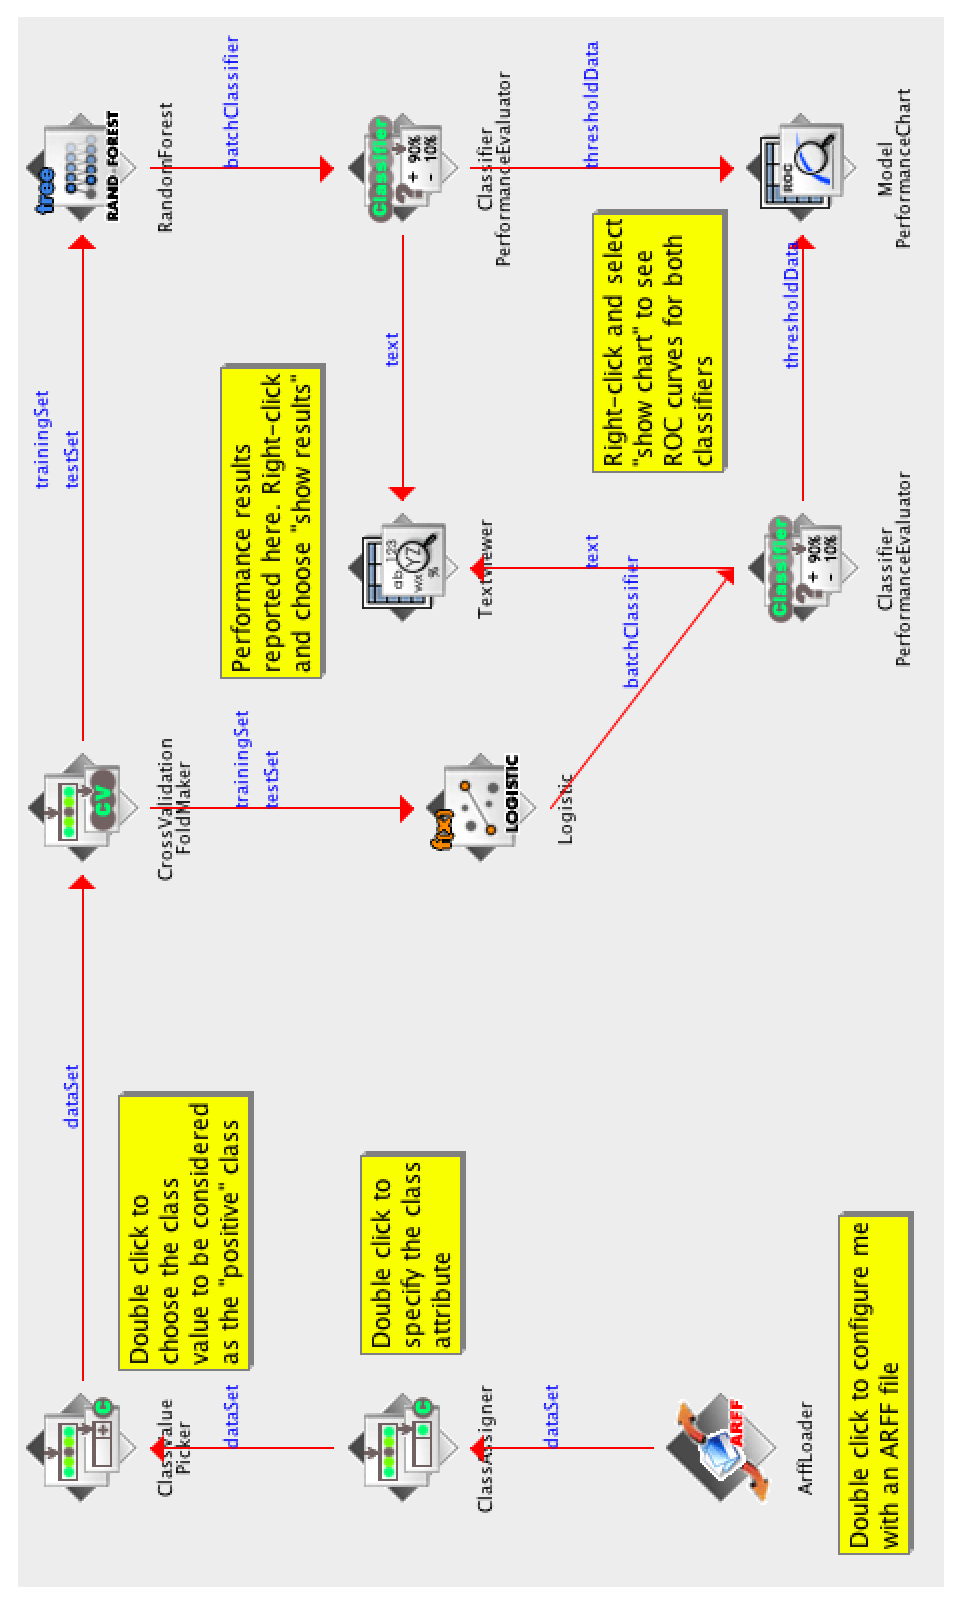
\includegraphics[angle=270,width=10cm]{images/knowledgeflow/example_multiple_roc.eps}
%	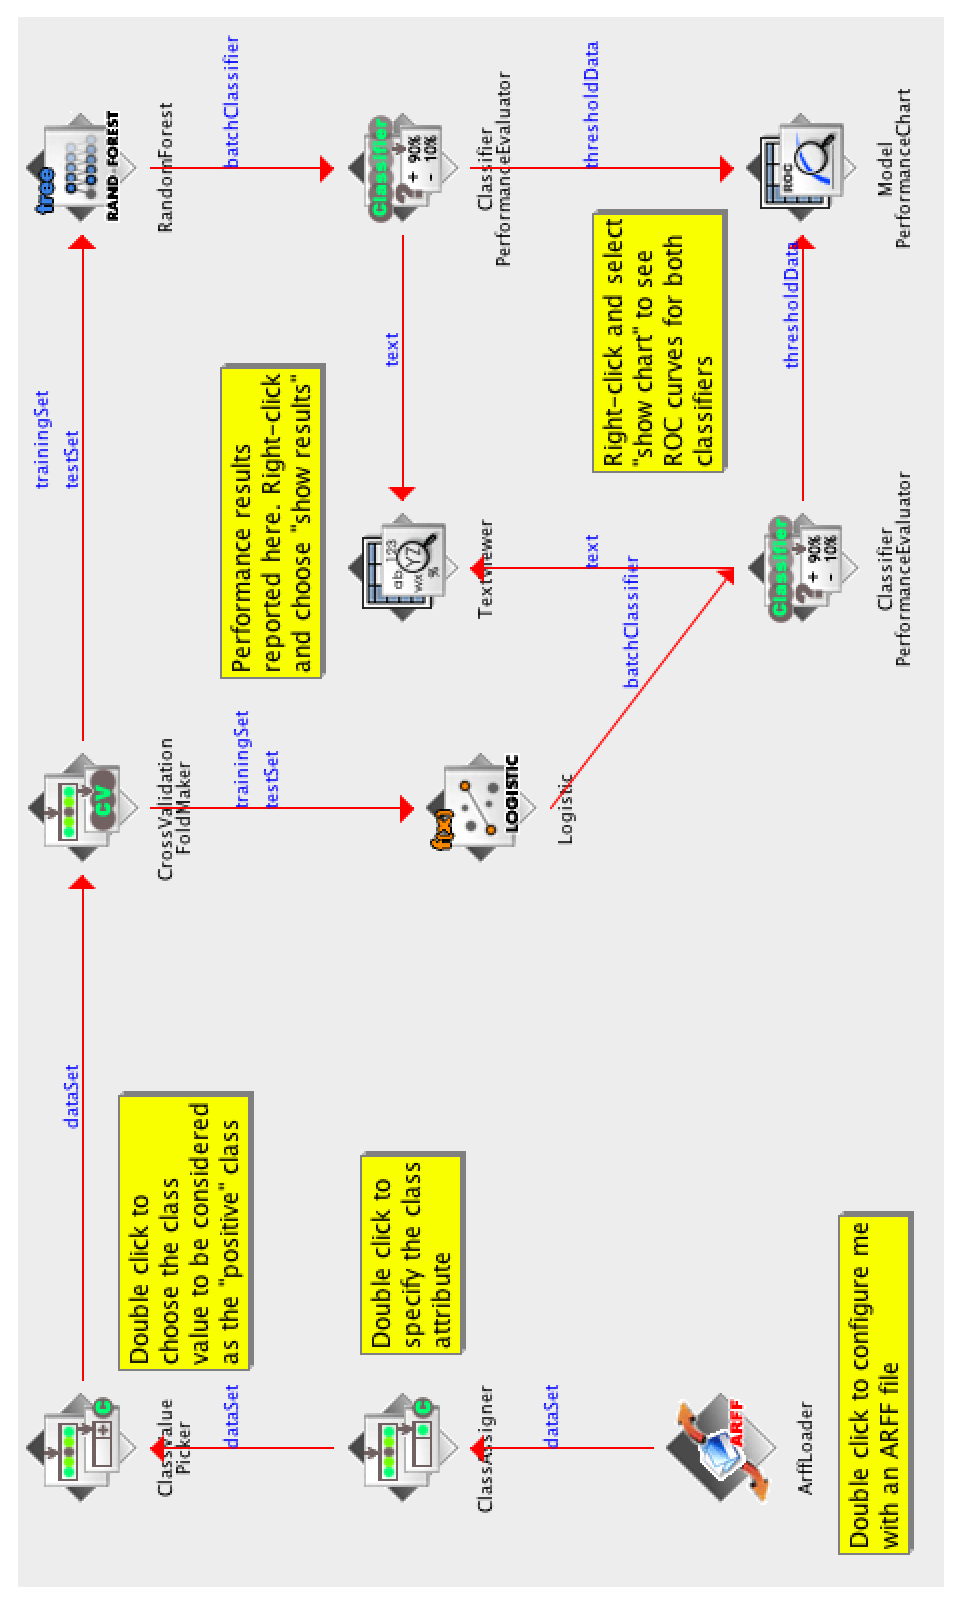
\epsfig{file=images/knowledgeflow/example_multiple_roc.eps,height=4cm}
\end{center}

\begin{itemize}
	\item Click on the DataSources entry in the \textit{Design}
          panel and choose \textit{ArffLoader} (the mouse pointer will
          change to a \textit{cross hairs}).

	\item Next place the ArffLoader step on the layout area by clicking
	somewhere on the layout (a copy of the ArffLoader icon will appear on
	the layout area).

	\item Next specify an ARFF file to load by first right clicking the mouse
	over the ArffLoader icon on the layout. A pop-up menu will
	appear. Select \textit{Configure} under \textit{Edit} in the list from this menu and
	browse to the location of your ARFF file.

	\item Next click the \textit{Evaluation} entry in the
          \textit{Design} panel and choose the \textit{ClassAssigner}
          (allows you to choose which column to be the class)
          step from the toolbar. Place this on the layout.

	\item Now connect the ArffLoader to the ClassAssigner: first right click
	over the ArffLoader and select the \textit{dataSet} under \textit{Connections} in
	the menu. A \textit{rubber band} line will appear. Move the mouse over the
	ClassAssigner step and left click - a red line labeled \textit{dataSet}
	will connect the two stepss.

	\item Next right click over the ClassAssigner and choose \textit{Configure} from
	the menu. This will pop up a window from which you can specify which
	column is the class in your data (last is the default).

	\item Next choose the \textit{ClassValuePicker} (allows you to
          choose which class label to be evaluated in the ROC)
          step from \textit{Evaluation}. Place this on
          the layout and right click over \textit{ClassAssigner} and
          select \textit{dataSet} from under \textit{Connections} in
          the menu and connect it with the \textit{ClassValuePicker}.

	\item Next grab a \textit{CrossValidationFoldMaker} step
          from \textit{Evaluation} and place it on the layout. Connect
          the ClassAssigner to the CrossValidationFoldMaker by right
          clicking over \textit{ClassAssigner} and selecting
          \textit{dataSet} from under \textit{Connections} in the
          menu.

	\item Next click on the \textit{Classifiers} entry in the
          \textit{Design} panel and choose the \textit{J48} step
          from the \textit{trees} sub-entry. Place a J48 step on
          the layout.

	\item Connect the CrossValidationFoldMaker to J48 TWICE by first choosing
	\textit{trainingSet} and then \textit{testSet} from the pop-up menu for the
	CrossValidationFoldMaker.

	\item Repeat these two steps with the RandomForest classifier.

	\item Next go back to \textit{Evaluation} and place a
	\textit{ClassifierPerformanceEvaluator} step on the layout. Connect J48
	to this step by selecting the \textit{batchClassifier} entry from the
	pop-up menu for J48. Add another \textit{ClassifierPerformanceEvaluator} for
	RandomForest and connect them via \textit{batchClassifier} as well.

	\item Next go to the \textit{Visualization} entry and place a 
	\textit{ModelPerformanceChart} step on the layout. Connect both 
	ClassifierPerformanceEvaluators to the ModelPerformanceChart by selecting 
	the \textit{thresholdData} entry from the pop-up menu for ClassifierPerformanceEvaluator.

	\item Now start the flow executing by pressing the
          \textit{play} button on the toolbar at the top of the
          window. Progress information for each step in the flow
          will appear in the \textit{Status} bar and \textit{Log} at
          the bottom of the window.
	
	\item Select \textit{Show plot} from the popup-menu of the 
	\textit{ModelPerformanceChart} under the \textit{Actions} section.
\end{itemize}

Here are the two ROC curves generated from the UCI dataset \textit{credit-g}, 
evaluated on the class label \textit{good}:

\begin{center}
	\epsfig{file=images/knowledgeflow/example_multiple_roc_output.eps,height=8.5cm}
\end{center}

%%%%%%%%%%%%%%%%%%%%%%%%%%%%%%%%%%%%%%%%%%%
% Example: processing data incrementally  %
%%%%%%%%%%%%%%%%%%%%%%%%%%%%%%%%%%%%%%%%%%%

\newpage
\subsection{Processing data incrementally}

Some classifiers, clusterers and filters in Weka can handle data
incrementally in a streaming fashion. Here is an example of training
and testing \textit{naive Bayes} incrementally. The results are sent
to a \textit{TextViewer} and predictions are plotted by a
\textit{StripChart} step. This example can be accessed from the
``Learn and evaluate naive Bayes incrementally'' entry of the popup menu that
appears when the ``templates'' button in the toolbar is clicked.

\begin{center}
  \includegraphics[angle=270,width=10cm]{images/knowledgeflow/IncrementalFlow.eps}
\end{center}

\begin{itemize}
        \item Expand the DataSources entry in the \textit{Design}
          panel and choose \textit{ArffLoader} (the mouse pointer will
          change to a \textit{cross hairs}).

	\item Next place the ArffLoader step on the layout area by clicking
	somewhere on the layout (a copy of the ArffLoader icon will appear on
	the layout area).

	\item Next specify an ARFF file to load by first right clicking the mouse
	over the ArffLoader icon on the layout. A pop-up menu will
	appear. Select \textit{Configure} under \textit{Edit} in the list from this menu and
	browse to the location of your ARFF file.

	\item Next expand the \textit{Evaluation} entry in the
          \textit{Design} panel and choose the \textit{ClassAssigner}
          (allows you to choose which column to be the class). Place
          this on the layout.

	\item Now connect the ArffLoader to the ClassAssigner: first right click
	over the ArffLoader and select the \textit{dataSet} under \textit{Connections} in
	the menu. A \textit{rubber band} line will appear. Move the mouse over the
	ClassAssigner step and left click - a red line labeled \textit{dataSet}
	will connect the two steps.

	\item Next right click over the \textit{ClassAssigner} and choose \textit{Configure} from
	the menu. This will pop up a window from which you can specify which
	column is the class in your data (last is the default).

        \item Now grab a \textit{NaiveBayesUpdateable} step from the \textit{bayes}
        section of the \textit{Classifiers} entry and place it on the layout.

        \item Next connect the \textit{ClassAssigner} to \textit{NaiveBayesUpdateable}
        using a \textit{instance} connection.

        \item Next place an \textit{IncrementalClassiferEvaluator} from the \textit{Evaluation}
        entry onto the layout and connect \textit{NaiveBayesUpdateable} to it using a
        \textit{incrementalClassifier} connection.

        \item Next place a \textit{TextViewer} step from the \textit{Visualization}
        entry on the Layout. Connect the \textit{IncrementalClassifierEvaluator} to
        it using a \textit{text} connection.

        \item Next place a \textit{StripChart} step from the \textit{Visualization}
        entry on the layout and connect \textit{IncrementalClassifierEvaluator} to it
        using a \textit{chart} connection.

        \item Display the \textit{StripChart's} chart by right-clicking over it and choosing
        \textit{Show chart} from the pop-up menu. Note: the \textit{StripChart} can be configured
        with options that control how often data points and labels are displayed.

        \item Finally, start the flow by pressing the \textit{play} button on the toolbar at the top of the window.        
\end{itemize}

\begin{center}
  \includegraphics[angle=270,width=12cm]{images/knowledgeflow/IncrementalChart.eps}
\end{center}

Note that, in this example, a prediction is obtained from naive Bayes
for each incoming instance {\bf before} the classifier is trained
(updated) with the instance. If you have a pre-trained classifier, you
can specify that the classifier {\bf not} be updated on incoming
instances by unselecting the check box in the configuration dialog for
the classifier. If the pre-trained classifier is a {\bf batch}
classifier (i.e. it is not capable of incremental training) then you
will only be able to test it in an incremental fashion.

\begin{center}
  \includegraphics[angle=270,width=12cm]{images/knowledgeflow/IncrementalClassifierConfig.eps}
\end{center}

\newpage
\section{Plugins}

\subsection{Flow components}
The KnowledgeFlow offers the ability to easily add new components via
a plugin mechanism. From Weka 3.7.2 this plugin mechanism has been
subsumed by the package management system and KnowledgeFlow plugins
are no longer installed in \verb=.knowledgeFlow/plugins= in the user's
home directory. Jar files containing plugin components for the
KnowledgeFlow need to be bundled into a package archive. Information
on the structure of a Weka package is given in the Appendix (Chapter
19). In order to tell the KnowledgeFlow which classes in the jar file
to instantiate as components, a second file called
\verb=PlugnManager.props= needs to be included in the top-level
directory of the package. This file contains key/value entries, where
the key specifies an interface or base class, and the value is a
comma-separated list of concrete implementations.  For example, if
we'd developed a new Knowledge Flow step called \verb=FunkyStep=, then
the PluginManager.props file would contain the following entry:

\begin{verbatim}
weka.knowledgeflow.steps.Step=weka.knowledgeflow.steps.FunkyStep
\end{verbatim}

If we had developed a new perspective (see the next section) called
\verb=FunkyPerspective=, then an entry such as the following would
make it appear in the Knowledge Flow (and Workbench).

\begin{verbatim}
weka.gui.Perspective=weka.gui.knowledgeflow.FunkyPerspective
\end{verbatim}


\subsection{Perspectives}
From Weka 3.7.4, the KnowledgeFlow offers a new type of plugin, called
a ``perspective'', that can take over the main UI and add major new
functionality. One example is the \textit{timeSeriesForecasting}
package. This package offer not only a plugin tab for the Explorer,
but also a plugin perspective for the KnowledgeFlow as well. Another
example is the \textit{scatterPlot3D} package which adds a 3D
visualization facility for datasets. Both these perspectives operate
on a set of instances. Instances can be sent to a perspective by
right-clicking over a configured \textit{DataSource} component and
choosing \textit{Send to perspective} from the popup menu.

\begin{center}
  \includegraphics[angle=270,width=12cm]{images/knowledgeflow/sendToPerspective.eps}
\end{center}

\begin{center}
  \includegraphics[angle=270,width=12cm]{images/knowledgeflow/scatterPlot3DPerspective.eps}
\end{center}

Several perspectives are built-in to Knowledge Flow and others, such
as the time series environment, can be installed as packages. The
built-in perspectives include: \textit{Attribute summary}, \textit{SQL
  Viewer} and \textit{Scatter plot matrix}. Which perspectives appear
in the toolbar can be configured by clicking the button shaped like a
cog in the upper left-hand corner of the main Knowledge Flow
window. If the Perspectives toolbar is not visible then it can be
shown/hidden by clicking the ``cog with arrow'' button in the main
toolbar at the top right-hand side of the main Knowledge Flow window.
